\section{Νέο περιφερειακό}
\label{sec:example2}

Για να παραχθεί ο επιθυμητός κώδικας που υλοποιεί βασικές λειτουργίες για κάποιο περιφερειακό, πρέπει πρώτα να έχουν φτιαχτεί 2 συγκεκριμένα αρχεία. Το πρώτο, είναι αυτό που γράφεται στην γλώσσα που αναλύεται στην \autoref{subsec:syntax_device}, και είναι αυτό το οποίο ουσιαστικά θα περιγράφει την εκάστοτε συσκευή. Το δεύτερο, είναι ένα πρότυπο αρχείο κώδικα C, το οποίο υλοποιεί τις επιθυμητές λειτουργίες, παίρνοντας ως ορίσματα συγκεκριμένες παραμέτρους. Στην παρούσα εργασία, τα αρχεία αυτά έχουν παραχθεί για τα 4 περιφερειακά που παρουσιάζονται στο \autoref{sec:supported} και άρα αν ο χρήστης επιθυμεί την προσθήκη κάποιου επιπλέον θα πρέπει να πραγματοποιήσει την ακόλουθη διαδικασία. Εδώ είναι σημαντικό να αναφερθεί, πως για να είναι σχετικά εύκολη η διαδικασία προσθήκης του περιφερειακού, ο χρήστης θα πρέπει να ελέγξει πως υπάρχει ο αντίστοιχος driver, και άρα ήδη υποστηρίζεται από το RIOT. Σε αντίθετη περίπτωση, τότε θα πρέπει ο χρήστης να γράψει από την αρχή τον driver, κάτι το οποίο είναι αρκετά περίπλοκο, και ξεφεύγει και από τα πλαίσια της παρούσας διπλωματικής.

Έστω λοιπόν ότι ο χρήστης θέλει να χρησιμοποιήσει τον αισθητήρα περιβάλλοντος BME280. Αν στο αρχείο (.con) όπου δηλώνονται οι συνδέσεις του κάθε περιφερειακού με τον μικροελεγκτή, συμπεριλάβει τον αισθητήρα αυτόν, τότε η εντολή για την παραγωγή κώδικα θα επιστρέψει το μήνυμα που φαίνεται στο \autoref{fig:error_message1}, καθώς δεν υπάρχει έτοιμη υλοποίηση.

\begin{figure}[!ht]
	\centering
	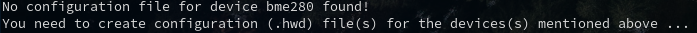
\includegraphics[width=1.0\textwidth]{./images/chapter6/error_message1.png}
	\caption{Μήνυμα για συσκευή που δεν υποστηρίζεται}
	\label{fig:error_message1}
\end{figure}

Το πρώτο βήμα που πρέπει να κάνει λοιπόν ο χρήστης, είναι να δημιουργήσει ένα .hwd αρχείο, όπου θα περιγράφει τα χαρακτηριστικά του αισθητήρα (σύμφωνα με τη γλώσσα που υλοποιήθηκε στην παρούσα εργασία).

Το περιεχόμενο του αρχείου θα μπορούσε να είναι το ακόλουθο.

\begin{lstlisting}
peripheral:
	name: bme280
	type: sensor
	operating_voltage: 3.3
	vcc: 3.3
	pins:
	- power:
		name: vcc
		number: 1
		type: 5v
	- power:
		name: gnd
		number: 2
		type: gnd
	- io_pin: -> sck-0
		name: sck
		number: 3
	- io_pin: -> miso-0
		name: miso
		number: 4
	- io_pin: -> mosi-0
		name: mosi
		number: 5
	- io_pin: -> cs-0
		name: cs
		number: 6
\end{lstlisting}

Έστω ότι ο χρήστης εκτελεί ξανά την εντολή για την παραγωγή του κώδικα. Αυτή τη φορά θα επιστρέψει το μήνυμα που φαίνεται στο \autoref{fig:error_message2}, καθώς δεν υπάρχει το πρότυπο αρχείο C. Η διαδικασία θα σταματήσει, ωστόσο θα δημιουργηθεί το πρότυπο αρχείο (με το όνομα του περιφερειακού) και θα έχει το ακόλουθο περιεχόμενο.

\begin{lstlisting}
void send_{{ peripheral_name[loop.index0] }}(void *arg)
{
	(void) arg;
	
	/* Name of the topic */
	char topic[32];
	sprintf(topic, "{{topic[loop.index0]}}");
	
	/* Allocate memory for the message to be published */
	char *msg = malloc(128);
	
	/*
	 * You need to fill the rest of this function. This function 
	 * should first initialize the sensor, get a measurement,
	 * and then publish it to the broker. 
	 */
	
	return NULL;
}
\end{lstlisting}

\begin{figure}[!ht]
	\centering
	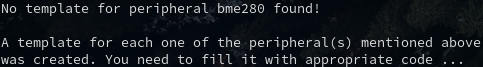
\includegraphics[width=0.8\textwidth]{./images/chapter6/error_message2.png}
	\caption{Μήνυμα για περιφερειακό για το οποίο δεν υπάρχει το πρότυπο αρχείο.}
	\label{fig:error_message2}
\end{figure}

Στο σημείο των σχολίων, ο χρήστης πρέπει να προσθέσει τον κώδικα με τον οποίο θα υλοποιηθούν οι επιθυμητές λειτουργίες. Στην περίπτωση αυτή, όπου πρόκειται για έναν αισθητήρα, θα πρέπει να γίνει πρώτα η αρχικοποίησή του, στη συνέχεια να πραγματοποιήσει μία μέτρηση, και να την κοινοποιήσει στον broker. Στην περίπτωση ενός ενεργοποιητή, θα πρέπει να γραφτεί κώδικας ώστε αρχικά να αποθηκεύεται το κοινοποιημένο μήνυμα, να γίνεται η αρχικοποίηση του ενεργοποιητή, και στη συνέχεια να πραγματοποιείται η κατάλληλη λειτουργία σύμφωνα με το μήνυμα που κοινοποιήθηκε.

Αφού συμπληρωθεί και αυτό το αρχείο, τότε πλέον το περιφερειακό αυτό υποστηρίζεται πλήρως, και άρα μπορεί να χρησιμοποιηθεί σαν όρισμα στη διαδικασία.
